\documentclass{article}

\usepackage[left=1.5cm, right=1.5cm, top=3cm, bottom = 3cm]{geometry}

\usepackage{amsmath}
\usepackage{amsfonts}
\usepackage{amssymb}
\usepackage{graphicx}
\usepackage{float}
\usepackage{indentfirst}
\usepackage{wrapfig}
\usepackage{latexsym}
\usepackage{hyperref}
\usepackage{feynmf}
\linespread{1.1}

% frequently used 3-vector notations
\newcommand{\mtp}{\mathbf{p}}
\newcommand{\mtq}{\mathbf{q}}
\newcommand{\mtk}{\mathbf{k}}
\newcommand{\pnx}{\mathbf{x}}
\newcommand{\pny}{\mathbf{y}}
\newcommand{\pnr}{\mathbf{r}}

% frequently use spin notations

\newcommand{\uspin}{\uparrow}
\newcommand{\dspin}{\downarrow}

\author{\emph{Fang Xie, Department of Physics \& IASTU, Tsinghua University}}
\title{{\bf{Boson Hubbard Model zero temperature phase diagram}}}
\date{\today}
\begin{document}
\maketitle
\section{Bose Hubbard Model Hamiltonian}
Hubbard model is the simplest strong correlated system. The original Hubbard model describes materials in which the electrons interact with each other strongly. Also, we can find similar system in the ultra cold atom system in optical lattice. The atoms can be either bosons or fermions, but it is easy to deal with bosons, so we talk about the bosons for simplicity.

The Hamiltonian of Boson-Hubbard Model is:
\begin{equation}
H = -w\sum_{\langle ij\rangle}b^\dagger_ib_j +\frac{U}{2}\sum_{i}b^\dagger_ib^\dagger_ib_ib_i - \mu \sum_i b^\dagger_i b_i
\end{equation}
The first term is the kinetic energy and $w$ is the wave function overlap between two lattice point:
$$
w = -\int d^3x\, \phi^*_i(\pnx)\left(-\frac{\nabla^2}{2m}+V(\pnx)\right)\phi(\pnx)
$$
The second term is the on-site repulsion energy; the third term is the chemical potential. Now we consider about the phase transition of this model at $T=0$. In the Grand Canonical theory, The system will stay at the ground state. So we should try to determine the ground state, and find out how it changes when we control the parameters, including $w$, $\mu$ and $U$.

\section{Perturbation approach of mean field approximation}
\subsection{Mean-Field Hamiltonian}
In this section we introduce a method which we call the mean field theory, to find the ground state and determine different phases of the system. Assume that the boson operator can be written as:
\begin{eqnarray}
b^\dagger_i& =& \psi^* + \delta b^\dagger_i\\
b_j &= & \psi + \delta b_j
\end{eqnarray}
Put these into the Hamiltonian and neglect the higher order terms like $\delta b^\dagger_i \delta b_j$, we get the {\bf{mean-field Hamiltonian}}:
\begin{eqnarray}
H_{MF} &=& -w \sum_{\langle ij\rangle}(\psi^* + \delta b^\dagger_i)(\psi+ \delta b_j) + \sum_i h_i \nonumber\\
&=& -w\sum_{\langle ij\rangle} \left( \psi^*b_j + b^\dagger_i \psi-\psi^*\psi \right) + \sum_i h_i\nonumber\\
&=& \sum_i \left( wZ\psi^*\psi -wZb^\dagger_i\psi -wZ\psi^*b_i +\frac{U}{2}n_i(n_i-1) - \mu n_i \right)
\end{eqnarray}
in which $h_i = Un_i(n_i-1)/2 -\mu n_i$ and $Z$ is the coordination number of the lattice. We can treat the field $\psi$ as a variational parameter and find the ground state under a group of given parameter.
\subsection{Mott-Insulator Phase}
Assumes that the potential well of the optical lattice is very deep, so the kinetic term is small compares to the interacting term $U$. So we can treat the kinetic term as a perturbation. 

First, we have to find the ground state when $w=0$. Since then the original Hamiltonian is decoupled, the mean field is exact:
\begin{equation}
|GS\rangle = | n(\mu)\rangle
\end{equation}
in which the occupying number on each site will be:
$$
n(\mu) = \left\{ \begin{array}{ll}
0 & \mu/U<0 \\
1 & 0<\mu/U<1\\
2 & 1<\mu/U<2\\
\vdots &\vdots
\end{array}\right.
$$
and when $\mu/U$ is an integer, there will be a two-fold degeneracy. Now we can write down the ground state energy when $w= 0$:
\begin{equation}
\frac{E_0}{M} = \frac{U}{2}n(\mu)(n(\mu)-1)-\mu n(\mu)
\end{equation}
We can find that each site is occupied by a number of bosons, which means that the bosons are localized. Since $\psi = \langle b_i \rangle$, obviously we can find that $\psi = 0$, which means the $U(1)$ symmetry of the Hamiltonian is not broken in this phase. This is the so called ``Mott-insulator'': particles cannot move to different sites, because it will cost too much energy.

\subsection{Second order perturbation and superfluid phase}
If we turn on the kinetic term $w$, we can calculate the perturbation. Clearly the first order perturbation energy is zero, so we need to find the second order energy:
\begin{eqnarray}
\frac{E^{(2)}}{M} &=& \sum_{m\neq n}\frac{|\langle GS|H_1|m\rangle|^2}{E_0-E_m}\nonumber\\
&=& wZ\psi^*\psi + w^2Z^2\psi^*\psi\left[\frac{n(\mu)+1}{\mu-Un(\mu)}+\frac{n(\mu)}{U(n(\mu)-1)-\mu}\right]
\end{eqnarray}
so we can find that the energy can be expressed as a function of $\psi$:
\begin{equation}
\frac{E_{MF}}{M} = \left[\frac{U}{2}n(\mu)(n(\mu)-1)-\mu n(\mu)\right] + r\psi^*\psi +\mathcal{O}(\psi^4)
\end{equation}
and the coefficient of the quadratic term $r$ is:
\begin{equation}
r = wZ + w^2Z^2\left[\frac{n(\mu)+1}{\mu-Un(\mu)}+\frac{n(\mu)}{U(n(\mu)-1)-\mu}\right] 
\end{equation}
Now if we control the parameters in our model to make $r<0$, and if we do the variational of $\psi$, we can find that the expectation value $\psi\neq 0$. The original global $U(1)$ symmetry is broken and we are in the superfluid phase. Clearly the phase boundary between M.I and S.F is given by:
\begin{equation}
0 = 1 + wZ \left[\frac{n(\mu)+1}{\mu-Un(\mu)}+\frac{n(\mu)}{U(n(\mu)-1)-\mu}\right]\,.
\end{equation}
\section{Phase diagram}
In this section we try to get the phase diagram of our boson Hubbard model. The equation of the phase boundary is given by Eq.(10), it is easy to get the diagram by Mathematica. For simplicity, we set $U = 1$ and solve the solution on a two-dimensional square lattice, on which $Z = 4$:
\begin{verbatim}
number[u_] := If[u < 0, 0, Floor[u] + 1];
F[w_, mu_] := 1 + 4 w ((number[mu] + 1)/(mu - number[mu]) + number[mu]/(number[mu] - 1 - mu));
Timing[ContourPlot[F[w, mu] == 0, {w, 0, 0.1}, {mu, -1, 5}, PerformanceGoal -> "Quality"]]
\end{verbatim}
and the result is:
\begin{figure}[!htp]
\centering
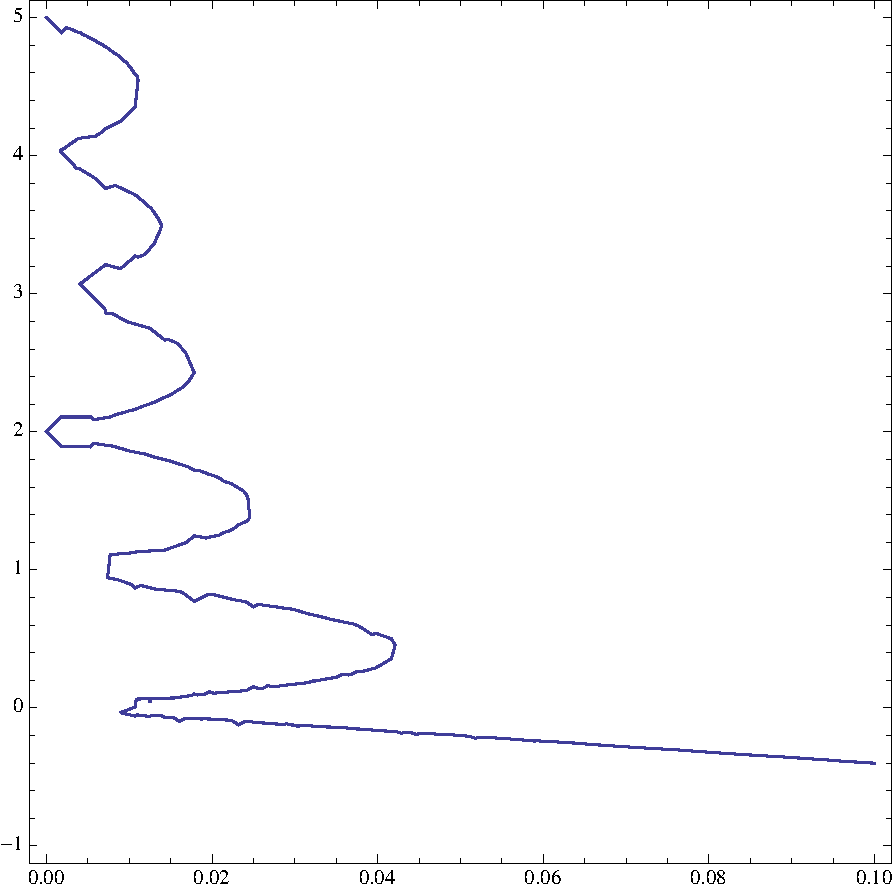
\includegraphics[width=8cm]{Pic1.pdf}
\caption{Phase diagram of Boson Hubbard Model at $T=0$. Obtained by mean field theory}
\end{figure}


\begin{thebibliography}{99}
\bibitem{a}{SUBIR SACHDEV: Quantum Phase Transition, 2011.}
\bibitem{b}{FISHER, M., WEICHMAN, P. B., GRINSTEIN, G., \& FISHER, D. S. (1989). Boson Localization and the Superfluid-Insulator Transition. Physical Review B, 40(1), 546–570.}
\end{thebibliography}

\end{document}








